\documentclass[11pt]{article}

% ---------------------------------------------------------------- packages
\usepackage[margin=1in]{geometry}
\usepackage{graphicx}
\usepackage{adjustbox}
\usepackage{booktabs}
\usepackage{amsmath}
\usepackage{caption}
\usepackage{subcaption}
\usepackage{float}
\usepackage[table]{xcolor}
\usepackage{hyperref}
\hypersetup{colorlinks=true, linkcolor=blue!60!black, urlcolor=blue!60!black,
            citecolor=blue!60!black}

% figures live under pipeline_rcf/out/figs/ relative to this file
\graphicspath{{pipeline_rcf/out/figs/}{figs/}}
\captionsetup{font=small, labelfont=bf}
\newcommand{\R}{$R^2$}

\title{\textbf{Predicting Compressive Strength and Optimal Replacement Level\\
for Recycled-Concrete-Fines Blended Cement from a Sparse Literature Dataset}}
\date{\today}

\begin{document}
\maketitle

\begin{abstract}
\noindent
We build a machine-learning pipeline to predict the compressive strength and the
optimal cement-replacement level of concrete blended with \textbf{recycled concrete
fines / recycled concrete powder} (RCF/RCP), from a dataset compiled from
\textbf{104 research papers}. As with the companion rice-husk-ash corpus, the
binding problem is data representation rather than model choice: strength values are
packed inside free-text cells as \emph{(replacement level $\times$ curing age)}
grids, spread across two differently-shaped sheets. Parsing and merging them
recovers \textbf{1825 data points across 85 papers}, of which 1284 also resolve a
curing age. A six-axis ablation shows that (i)~absolute strength across papers is
unpredictable (\R{}~$=-0.18$) but becomes learnable once the paper's own control
strength is supplied; (ii)~unlike the smaller RHA corpus, \emph{added features help
here}---chemistry and canonicalised categoricals both improve generalization at
44~papers where they overfit at 23; and (iii)~text embeddings still provide no
reliable gain. A tuned, monotonically-constrained gradient-boosted model reaches
\textbf{\R{}~$=0.448\pm0.175$, MAE~$=9.9$\,MPa}. That number should be read against
a hard \textbf{noise ceiling of \R{}~$=0.80$} which we quantify: 180 of the 260
(paper, level, age) cells contain several distinct mixes whose activation treatment
the dataset does not record. Finally, the optimal-replacement target turns out to be
ill-posed rather than merely hard---a paper's reported optimum and the argmax of its
\emph{own} strength table disagree by 14~percentage points at $r=0.43$, and for 62\%
of papers the strongest mix measured is the 0\% control.
\end{abstract}

% ============================================================================
\section{Introduction}
Recycled concrete fines (RCF), also reported as recycled concrete powder (RCP), are
the fine fraction left over when waste concrete is crushed. Using them to replace
part of the Portland cement in a new mix diverts a low-value waste stream and cuts
the $\mathrm{CO_2}$ footprint of the binder. The two engineering quantities of
interest are the \textbf{compressive strength} of the resulting concrete and the
\textbf{optimal replacement level}. Our goal is a predictive model for both, trained
on a dataset hand/LLM-extracted from the literature.

This report deliberately mirrors the methodology of our earlier study on rice husk
ash (RHA), so that the two materials can be compared on equal terms. Section~9
draws that comparison out; the short version is that RCF has roughly twice the
usable data and behaves quite differently as a material.

% ============================================================================
\section{The Dataset: What It Actually Contains}
The source workbook \texttt{Master\_sheet\_RCF.xlsx} has \textbf{two sheets}, and
that is its most important structural property.

\textbf{\texttt{Sheet1}} holds 225 columns over 105 data rows under a
\textbf{four-row hierarchical header}: super-banner ($\rightarrow$ \textsc{paper
metadata}/\textsc{input}/\textsc{output}), category, feature (55 features), and a
sub-field. Every feature is split into four columns---\texttt{Extracted Value},
\texttt{Unit}, \texttt{Source Type}, \texttt{Exact Evidence}---of which only the
first two carry predictive information. The first five columns are single-level
metadata (title, authors, journal, year, DOI), so $5 + 55\times4 = 225$. One paper
appears twice under different capitalisation, leaving \textbf{104 unique papers}.

\textbf{\texttt{Experimental Matrix}} is a flat six-column, 1162-row table that is
\emph{already exploded to one row per mix}, carrying \texttt{Mix ID},
\texttt{Replacement Level}, \texttt{Activation Method}, \texttt{Key Processing
Parameters} and \texttt{Reported Strength}. It covers 103 of the 104 papers and is
joined on title.

Two traps are specific to this workbook and both are silent failure modes:

\begin{itemize}\itemsep2pt
  \item \textbf{Missing values are the literal string \texttt{"NULL"}}, very often
        with a trailing parenthetical---\texttt{NULL (Note: the paper reports
        water/cement (w/c) ratio\dots)}. An equality test against \texttt{"NULL"}
        keeps those strings as data.
  \item \textbf{Units are inconsistent within a single column.} \texttt{Specific
        Surface Area} alone appears as m$^2$/kg, m$^2$/g and cm$^2$/g;
        \texttt{Bulk Density} as kg/m$^3$ and g/cm$^3$; the strength column
        includes one paper reporting psi and one reporting kg/cm$^2$. Values must
        be converted \emph{before} any plausibility filter, or a range guard
        silently deletes two thirds of a column.
\end{itemize}

Among the 104 papers, 93 report a compressive strength, 92 declare their
replacement levels, and 66 report an optimum. \textbf{Two papers are excluded as
out of scope} (logged to \texttt{excluded\_papers.csv}): both replace
\emph{aggregate} rather than cement, so their ``replacement level'' does not mean
the same thing as everyone else's, and pooling them would reintroduce exactly the
confound that makes framing~A unlearnable.

Sparsity is uneven rather than uniform. Among the 85 papers that yield strength
data, availability of the 30 retained features ranges from 100\%
(material family) and 97\% (processing method) down to 8\% (BET surface) and 6\%
(amorphous content)---that is, \textbf{0--94\% missing, with 18 of the 30 features
more than half missing} (Figure~\ref{fig:avail}).

\begin{figure}[H]
  \centering
  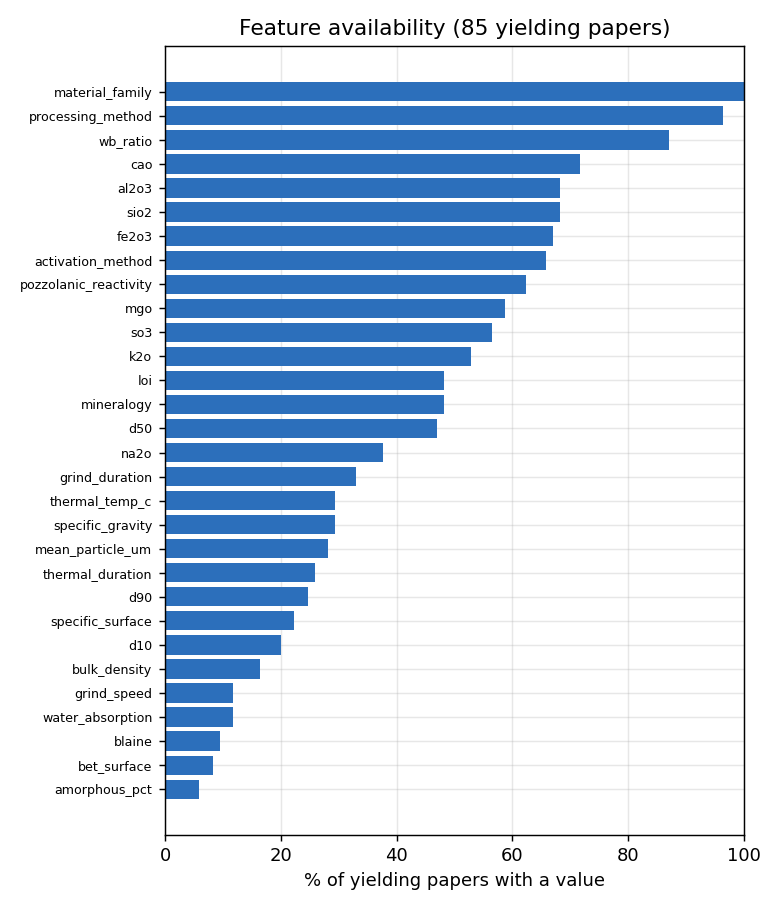
\includegraphics[width=0.5\textwidth]{data_availability.png}
  \caption{Per-feature availability among the 85 yielding papers. Material family,
  processing method and w/b are well populated; fineness measures (BET, Blaine,
  specific surface) and amorphous content are scarce. The dataset is larger than
  the RHA corpus but no less sparse.}
  \label{fig:avail}
\end{figure}

% ============================================================================
\section{Data Representation: Parsing Two Sheets Into One Table}
\label{sec:parse}
Each \texttt{Sheet1} strength cell encodes a \emph{grid} of measurements---and
sometimes a third w/b axis---in one of $\sim$16 textual layouts, for example
\begin{quote}\small\ttfamily
Ref (0\%): / 2 days: 26.6 $\pm$ 0.89 / 28 days: 45.8 $\pm$ 1.45 \dots\\
w/b 0.4: / 0\% RP: \~{}48.5 / 15\% RP: \~{}47.3 \dots\\
3-Day: 33.2 (MA20), 18.1 (MA50), 3.4 (MA100) \dots
\end{quote}
We built a line-oriented, context-carrying parser
(\texttt{02\_parse\_explode.py}) that resolves, for each value, a replacement level
and---where stated---a curing age, from an inline qualifier, a segment header, or
persistent line context. It reads \emph{both} sheets into one schema and
de-duplicates on the measurement itself. Precision safeguards include:
\begin{itemize}\itemsep2pt
  \item unsigned number matching, since a leading \texttt{-} is always a separator
        in this corpus;
  \item \textbf{reading the strength only from the value zone of an item.} This is
        not a detail. In \texttt{R20: 48.1} and \texttt{N-0.50-0: 28.5} the mix
        label contains numbers, and treating the item as a flat string makes the
        parser report strengths of 20 and 0.50\,MPa. Items are first split into
        \texttt{label: value} or \texttt{value (label)}; two such bugs cost roughly
        0.2 of \R{} until they were found by hand-checking parsed rows against raw
        cells;
  \item a \textbf{per-paper whitelist}: a resolved level must match one of the
        paper's declared \texttt{Cement Replacement Level(s)} (plus 0 for the
        control), which rejects mis-read mix IDs such as \texttt{MFP400} and
        \texttt{Series 7};
  \item unit conversion (psi $\times0.00689476$, kg/cm$^2$ $\times0.0980665$) and
        physical clamps ($0\le\%\le100$, $0<\text{age}\le400$\,d,
        $0.5\le\text{MPa}\le250$).
\end{itemize}

This recovers \textbf{1825 data points across 85 of the 102 in-scope papers}---976
from the \texttt{Sheet1} grids and 849 from the Experimental Matrix
(Figures~\ref{fig:yield} and~\ref{fig:src}). \textbf{1284 points over 57 papers}
also resolve a curing age, 384 of them at the standard 28-day age. The 445 logged
parse failures are
overwhelmingly cells that report only a \emph{relative} change
(\texttt{3-day: +18\%, 28-day: +16\%}), a bare number list, or a figure reference,
and are genuinely unrecoverable without the source PDFs.

\paragraph{Curing age is not assumed.} Only 458 of the 1162 matrix rows state an
age. Treating the rest as 28-day measurements would be fabrication, so they are
retained with \texttt{age\_known = False} and excluded from the main modelling
table; Study~6 then tests that assumption empirically rather than baking it in.

\begin{figure}[H]
  \centering
  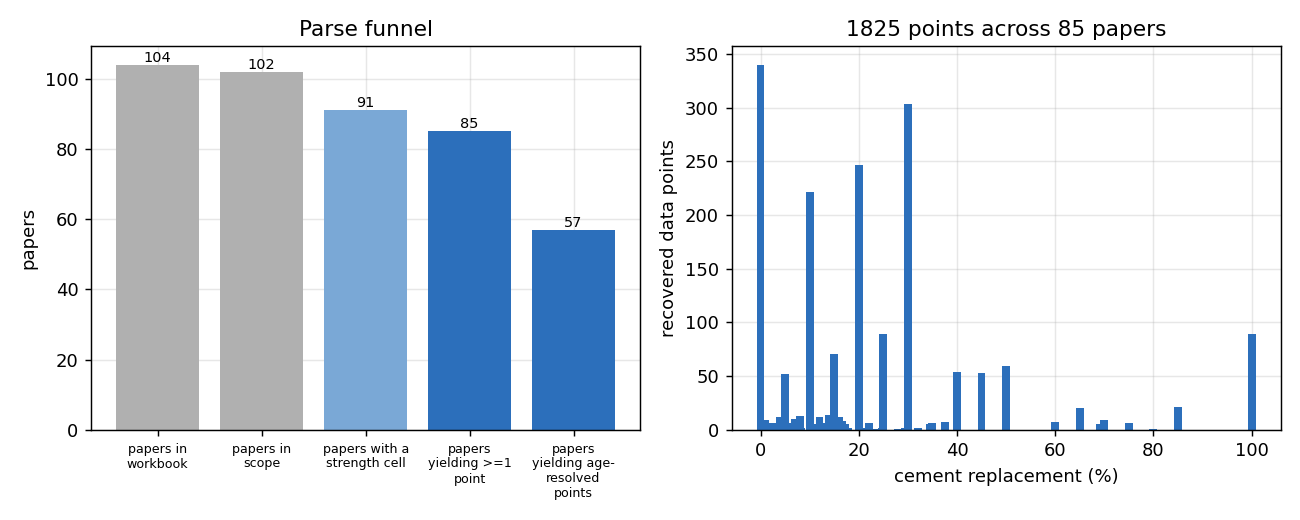
\includegraphics[width=0.92\textwidth]{parse_yield.png}
  \caption{Parse funnel (left) and the distribution of recovered points by
  replacement level (right). The corpus is concentrated at 10--30\% replacement,
  with a long tail out to 100\%.}
  \label{fig:yield}
\end{figure}

\begin{figure}[H]
  \centering
  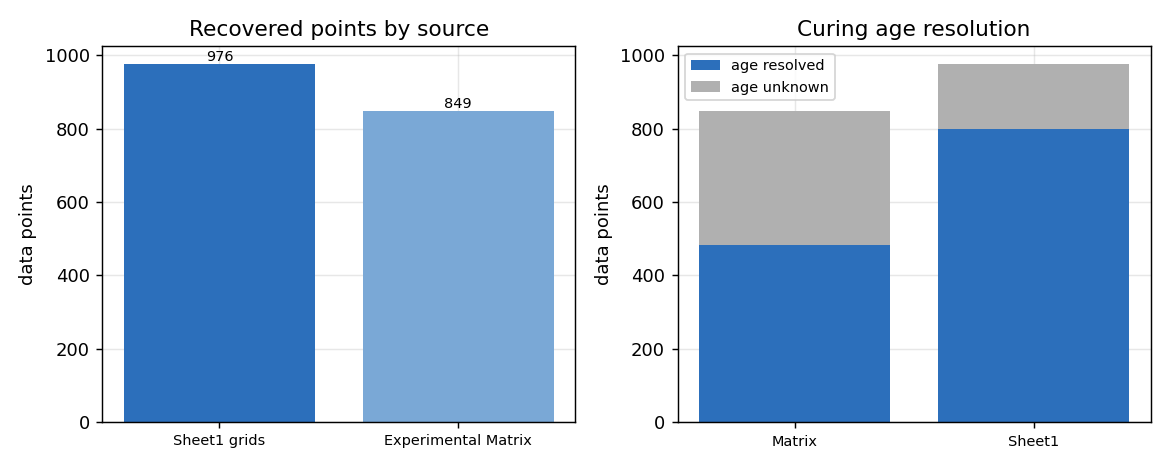
\includegraphics[width=0.92\textwidth]{sources.png}
  \caption{The two sheets contribute comparable numbers of points (976 and 849),
  but differ in what they resolve: 800 of the 976 \texttt{Sheet1} points (82\%)
  state a curing age, against 484 of the 849 matrix points (57\%). Both sources are
  needed---Study~6 shows that training on the matrix alone costs more than half the
  achievable \R{}.}
  \label{fig:src}
\end{figure}

\paragraph{Checks against expected physics.} Both checks must be made \emph{within}
a paper: a raw cross-paper average is dominated by mix type---the parsed corpus
spans 0.6\,MPa pastes to a 184\,MPa UHPC, and 0.6--108\,MPa among the age-resolved
rows these panels use---rather than by the variable of interest.
Normalising each \emph{(paper, replacement level)} series by its own 28-day value,
strength does rise with curing age: 77\% of pre-28-day points fall below their own
series' 28-day value and 83\% of later points exceed it, with the median ratio
climbing 0.62 (2\,d) $\rightarrow$ 0.83 (7\,d) $\rightarrow$ 1.00 (28\,d)
$\rightarrow$ 1.12 (90\,d). The one-day point is an exception, sitting at 0.87
rather than below the two-day value; it is drawn from a different subset of series
(only some papers report a one-day strength at all) and is a composition effect
rather than a reversal of the trend.

The strength-versus-replacement shape is where RCF differs most from RHA. Of the 31
papers reporting at least three distinct levels at 28\,d, only 7 (23\%) peak at an
interior level, while \textbf{22 (71\%) are highest at the lowest level tested} and
2 (6\%) are still rising at the highest. For this material, replacing cement
usually just costs strength---consistent with recycled concrete powder being far
less pozzolanic than rice husk ash and acting largely as a filler. That fact drives
the negative result in Section~\ref{sec:opt}.

\begin{figure}[H]
  \centering
  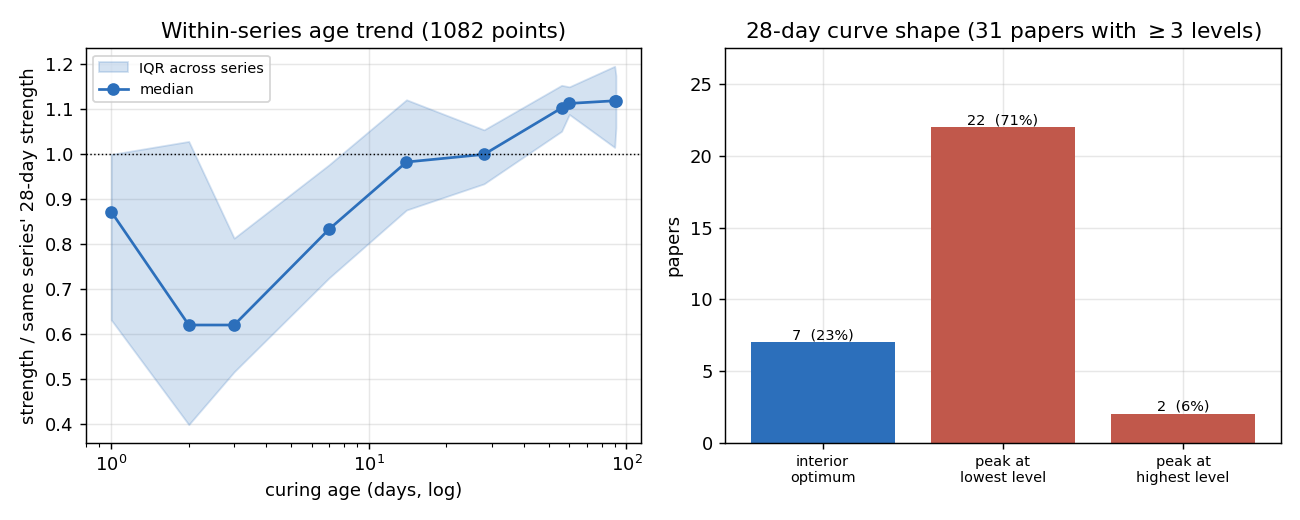
\includegraphics[width=0.9\textwidth]{cs_curves.png}
  \caption{Physics checks on the parsed data, computed within papers.
  \textbf{Left:} each \emph{(paper, replacement level)} series is normalised by its
  own 28-day strength; the median rises with age (shaded band is the IQR across
  series). The 1-day point breaks the pattern because a different, smaller set of
  series reports it. \textbf{Right:} the 28-day strength-vs-replacement curve has
  an interior optimum in only 23\% of papers; in 71\% the best level tested is the
  lowest one, frequently the 0\% control.}
  \label{fig:curves}
\end{figure}

% ============================================================================
\section{Feature Engineering}
Numeric cells are parsed as the mean of the numbers they contain, but only after
\textbf{unit normalisation} and inside a \textbf{physical range guard}. The guard
is load-bearing rather than cosmetic: the w/b cell \texttt{RC: 0.41 / C30R: 0.45 /
C100R: 0.48} contains 30 and 100 from the mix labels, and an unguarded mean reports
a water/binder ratio of 26.

High-cardinality free text is \textbf{canonicalized} into compact categoricals:
activation method $\in\{$none, thermal, \emph{carbonation}, mechanical, chemical,
multiple, other$\}$---carbonation is given its own level rather than being folded
into a generic ``other'', because CO$_2$ curing is a central RCF-specific
treatment; processing method $\in\{$crushing, milling, thermal, combined, other$\}$;
material family $\in\{$powder, fines, paste, cdw, aac, other$\}$, which folds the 90
free-text \texttt{Material Type} spellings together; and pozzolanic reactivity as an
ordinal, with negative markers tested first so that ``limited pozzolanic
reactivity'' does not score as high. We deliberately apply \textbf{no imputation}
for the tree models, which handle missing values natively; imputers are evaluated
separately in Study~4 and only ever fit \emph{inside} each cross-validation split.

% ============================================================================
\section{Methodology}
Because rows from the same paper are strongly correlated, all evaluation uses
\textbf{grouped cross-validation by paper}: no paper appears in both training and
test. Given the sample size, a single split is unreliable, so we report the mean and
standard deviation of \textbf{repeated grouped hold-out}
(\texttt{GroupShuffleSplit}, 30\% of papers held out, 40 repeats). We compare three
target framings:
\begin{description}\itemsep2pt
  \item[A. Absolute strength, all papers] predict MPa directly from RCF features.
  \item[B. Relative-to-control] predict strength normalized by the paper's 0\%
        control.
  \item[C. Absolute strength given control] predict the RCF-blend strength using
        the paper's control (0\%) strength at the same age as an additional
        input---always known in practice, hence not leakage. Control rows are
        excluded from evaluation to avoid a trivial identity.
\end{description}
Framing~C is evaluated on \textbf{823 blend rows over 44 papers}.

\paragraph{A noise ceiling worth stating up front.}
\label{sec:ceiling}
180 of the 260 \emph{(paper, replacement level, age)} cells in framing~C contain
\emph{more than one mix}---different activation treatments, and sometimes different
w/b ratios, at the same coordinate. Their spread is irreducible for any model that
cannot observe the treatment, and decomposing the variance puts a hard ceiling of
\textbf{\R{}~$=0.80$} on this task as posed. Every \R{} below should be read against
0.80, not against 1.0.

% ============================================================================
\section{Ablation Study}
\label{sec:abl}
We ablate six axes. All numbers are repeated grouped hold-out (mean\,$\pm$\,std)
over 40 repeats, except four rows noted with $^{\dagger}$ where 36--39 repeats
survived (a split is discarded when a fold ends up with no usable rows). Because
those rows are averaged over an easier subset of splits, \emph{their RMSE is not
comparable} to the 40-repeat rows; comparisons within a study are otherwise
like-for-like.

\paragraph{Study 1 --- Target framing.}
Absolute strength across papers is \emph{unpredictable} (\R{}~$=-0.184$): the
corpus mixes pastes, mortars and normal concrete, spanning
\textbf{0.6--108\,MPa} over the 1284 age-resolved rows framing~A is scored on,
and those baseline levels are set by mix factors absent from the data. (The
184\,MPa corpus maximum quoted in Section~\ref{sec:parse} is \emph{not} in this
set---that paper states no curing age, so it never enters an age-dependent
framing.) Supplying the control strength (framing~C) makes the RCF effect learnable
(Table~\ref{tab:s1}).

\begin{table}[H]\centering\small
\caption{Study 1: target framing (XGBoost, all structured features).}
\label{tab:s1}
\begin{tabular}{lrrrr}
\toprule
Framing & \R{} & std & RMSE & MAE \\
\midrule
\rowcolor{green!12}C: blend $\mid$ control strength & $0.341$ & $0.207$ & $14.18$ & $10.77$ \\
B: relative-to-control & $-0.170$ & $0.234$ & $0.32$ & $0.24$ \\
A: absolute, all papers & $-0.184$ & $0.320$ & $20.30$ & $16.05$ \\
\bottomrule
\end{tabular}
\end{table}

\paragraph{Study 2 --- Model.}
The tree ensembles are tightly bunched and all clearly beat the mean baseline;
HistGradientBoosting leads on the mean, with ExtraTrees, Random Forest,
GradientBoosting and XGBoost within 0.04 of it---well inside the run-to-run spread
of $\sigma\approx0.17$--$0.22$, so this ordering is not by itself reliable
(Table~\ref{tab:s2}). What \emph{is} decisive is the failure of the non-tree
candidates: Ridge (\R{}~$=-23.1$) and a small MLP (\R{}~$=-229$) are catastrophic on
this tiny, collinear, missing-laden matrix, and the stacked ensemble is dragged
below zero by its Ridge component. Section~\ref{sec:final} therefore searches over
the two gradient-boosted candidates rather than picking a winner here.

\paragraph{Study 3 --- Feature set.}
This is where RCF departs from the RHA corpus. There, the three-feature base set won
outright and \emph{every} added group hurt. Here, \textbf{added features help}: the
canonicalised categoricals lift \R{} from $0.311$ to $0.373$ and chemistry to
$0.350$ (Table~\ref{tab:s3}, Figure~\ref{fig:ablfeat}). With 44 papers rather than
23, the model can afford them. Text embeddings still cannot be justified---MiniLM
and TF-IDF both land \emph{below} the plain base set.

\begin{table}[H]\centering\small
\begin{minipage}{0.46\textwidth}\centering
\caption{Study 2: model (framing C, all features).}
\label{tab:s2}
\begin{tabular}{lrr}
\toprule
Model & \R{} & RMSE \\
\midrule
\rowcolor{green!12}HistGB$^{\dagger}$ & $0.384$ & $13.67$ \\
ExtraTrees & $0.371$ & $13.89$ \\
GradientBoosting & $0.353$ & $14.00$ \\
Random Forest & $0.353$ & $13.98$ \\
XGBoost & $0.341$ & $14.18$ \\
Stack (RF+XGB+Ridge) & $-0.028$ & $16.87$ \\
Mean baseline & $-0.080$ & $18.42$ \\
Ridge & $-23.1$ & $59.69$ \\
MLP (64,32) & $-229.2$ & $167.55$ \\
\bottomrule
\end{tabular}

{\scriptsize $^{\dagger}$39 of 40 repeats; RMSE not strictly comparable.}
\end{minipage}\hfill
\begin{minipage}{0.5\textwidth}\centering
\caption{Study 3: feature set (framing C, XGBoost).}
\label{tab:s3}
\begin{tabular}{lrr}
\toprule
Feature set & \R{} & RMSE \\
\midrule
\rowcolor{green!12}base + categorical & $0.373$ & $13.80$ \\
base + fineness & $0.370$ & $13.84$ \\
base + all numeric & $0.356$ & $13.98$ \\
base + chemistry & $0.350$ & $14.06$ \\
all structured & $0.341$ & $14.18$ \\
all + MiniLM text & $0.313$ & $14.39$ \\
base [repl, age, control] & $0.311$ & $14.48$ \\
all + TF-IDF text & $0.310$ & $14.46$ \\
base + processing & $0.272$ & $14.77$ \\
base + mix descriptors & $0.268$ & $14.90$ \\
\bottomrule
\end{tabular}
\end{minipage}
\end{table}

\paragraph{Study 4 --- Imputation.}
No imputer beats native NaN handling on like-for-like terms. MICE posts the highest
mean (\R{}~$=0.362$) but completed only 36 of 40 repeats, and median and KNN
completed 39 while scoring \emph{below} native; since none improves \R{} reliably
and each adds a fitted component that must be re-fit inside every split, we keep
\textbf{native handling} (Table~\ref{tab:s4}).

\paragraph{Study 5 --- Physics priors.}
Adding \textbf{monotone constraints}---strength non-decreasing in curing age and in
control strength---gives a consistent gain, $0.311\rightarrow0.339$
(Table~\ref{tab:s5}). Unlike the RHA study, this is not an XGBoost-only capability:
scikit-learn's \texttt{HistGradientBoostingRegressor} supports
\texttt{monotonic\_cst} as well, so the prior does not constrain the model choice.

\begin{table}[H]\centering\small
\begin{minipage}{0.46\textwidth}\centering
\caption{Study 4: imputation (framing C).}
\label{tab:s4}
\begin{tabular}{lrr}
\toprule
Scheme & \R{} & RMSE \\
\midrule
XGB + MICE$^{\dagger}$ & $0.362$ & $13.87$ \\
\rowcolor{green!12}XGB + native & $0.341$ & $14.18$ \\
XGB + median$^{\dagger}$ & $0.298$ & $14.59$ \\
XGB + KNN$^{\dagger}$ & $0.297$ & $14.59$ \\
Ridge + median & $-23.1$ & $59.69$ \\
\bottomrule
\end{tabular}

{\scriptsize $^{\dagger}$36--39 of 40 repeats; RMSE not comparable to the
native row.}
\end{minipage}\hfill
\begin{minipage}{0.5\textwidth}\centering
\caption{Study 5: physics priors (base features).}
\label{tab:s5}
\begin{tabular}{lrr}
\toprule
Prior & \R{} & RMSE \\
\midrule
\rowcolor{green!12}monotone(age, control) & $0.339$ & $14.10$ \\
log + monotone & $0.327$ & $14.17$ \\
log-target & $0.311$ & $14.44$ \\
plain & $0.311$ & $14.48$ \\
\bottomrule
\end{tabular}
\end{minipage}
\end{table}

\paragraph{Study 6 --- Which rows to train on.}
This axis has no counterpart in the RHA study; it exists because the RCF workbook
has two sources and a large pool of rows whose curing age never resolved. Here
\emph{only the training rows vary}---the held-out rows are identical in every
variant---so these \R{} values are directly comparable to one another, which they
would not be if the evaluation set changed too. Three results
(Table~\ref{tab:s6}):
\begin{itemize}\itemsep2pt
  \item \textbf{Averaging the duplicate mixes} in training is the single largest
        gain in the study, $0.341\rightarrow0.388$. This is the noise ceiling of
        Section~\ref{sec:ceiling} showing up as a modelling choice: when several
        treatments share one coordinate, their mean is a better training target
        than the individual points.
  \item \textbf{Both sources are needed.} Training on the Experimental Matrix alone
        collapses to $0.160$; the \texttt{Sheet1} grids alone reach $0.317$;
        together, $0.341$. The two halves are of similar size (380 and 443 of the
        823 rows, covering 30 and 34 of the 44 papers), so this is not simply a
        row-count effect: the matrix half is far more \emph{redundant}, its 380
        rows occupying only 100 distinct (paper, level, age) coordinates against
        the grids' 201, because the matrix lists many mixes per coordinate.
  \item \textbf{Assuming 28\,d for the age-unknown rows is neutral}
        ($0.341\rightarrow0.344$, well within $\sigma=0.21$). The assumption buys
        nothing, so we do not make it.
\end{itemize}

\begin{table}[H]\centering\small
\caption{Study 6: training data (framing C, XGBoost; held-out rows identical
across variants).}
\label{tab:s6}
\begin{tabular}{lrrr}
\toprule
Training set & \R{} & std & RMSE \\
\midrule
\rowcolor{green!12}duplicate mixes averaged & $0.388$ & $0.166$ & $13.69$ \\
$+$ age-unknown rows as 28\,d & $0.344$ & $0.210$ & $14.14$ \\
both sources (reference) & $0.341$ & $0.207$ & $14.18$ \\
\texttt{Sheet1} rows only & $0.317$ & $0.192$ & $14.42$ \\
matrix rows only & $0.160$ & $0.265$ & $15.98$ \\
\bottomrule
\end{tabular}
\end{table}

\begin{figure}[H]
  \centering
  \begin{subfigure}{0.49\textwidth}
    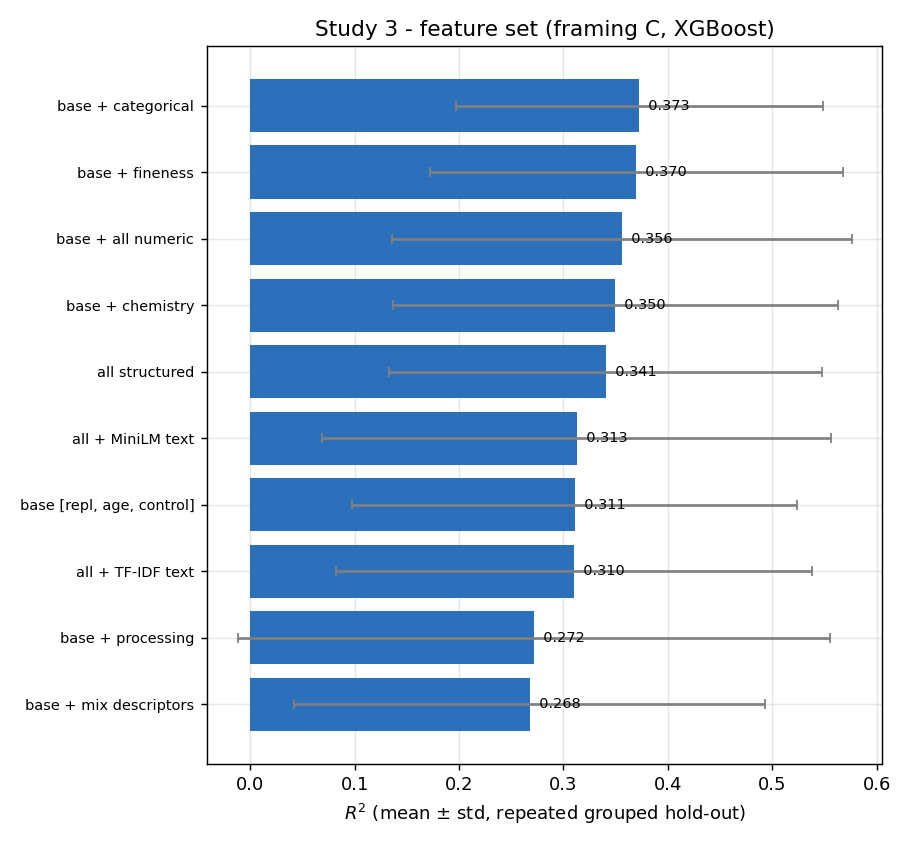
\includegraphics[width=\linewidth]{abl_features.png}
    \caption{Study 3 --- feature set.}
    \label{fig:ablfeat}
  \end{subfigure}\hfill
  \begin{subfigure}{0.49\textwidth}
    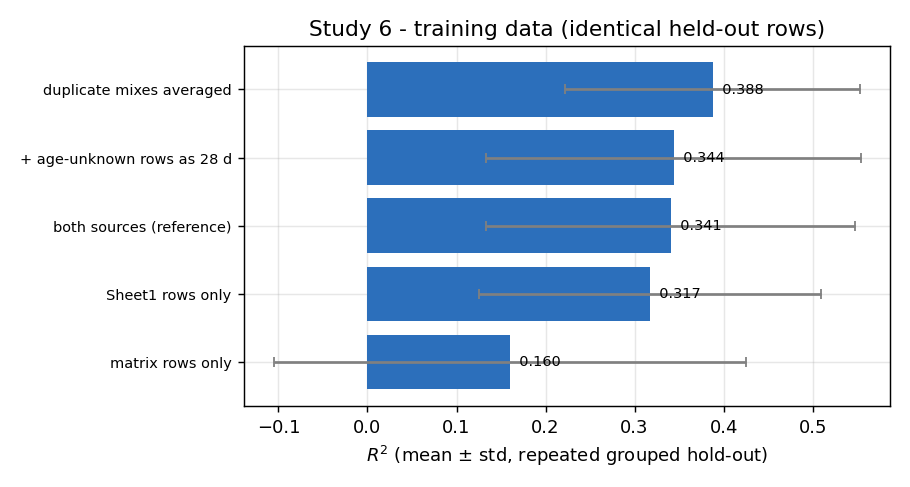
\includegraphics[width=\linewidth]{abl_data.png}
    \caption{Study 6 --- training data.}
    \label{fig:abldata}
  \end{subfigure}
  \caption{The two ablation axes where RCF behaves differently from RHA. Bars are
  mean\,$\pm$\,std over 40 repeated grouped hold-outs.}
\end{figure}

% ============================================================================
\section{Final Model and Results}
\label{sec:final}
Rather than hand-pick the ablation winners, we searched the architecture space they
opened up: \{HistGB, XGBoost\} $\times$ five feature sets $\times$ \{average
duplicate mixes in training or not\} $\times$ \{monotone or not\}, 40 configurations
each scored over the same 40 repeated grouped hold-outs
(\texttt{architecture\_search.csv}). Averaged over everything else, each axis moves
\R{} by a small but consistent amount: features \texttt{base+cat+chem} $0.410$ vs
\texttt{base} $0.355$; monotone $0.388$ vs unconstrained $0.378$; averaging
duplicates $0.386$ vs not $0.379$; and the two model families are indistinguishable
(HistGB $0.383$, XGBoost $0.382$). The best single configuration was XGBoost on
\texttt{base + categorical + chemistry}, training on averaged duplicates, with
monotone constraints. A 108-point hyper-parameter grid over that configuration then
selected a shallow, heavily-regularized model (\texttt{max\_depth}=2,
\texttt{learning\_rate}=0.1, 500 trees, \texttt{min\_child\_weight}=5,
\texttt{reg\_lambda}=3.0).

\begin{center}\small
\begin{tabular}{lccc}
\toprule
 & \R{} & RMSE (MPa) & MAE (MPa) \\
\midrule
\textbf{Final model} (repeated grouped hold-out) & $\mathbf{0.448\pm0.175}$ & $\mathbf{12.9}$ & $\mathbf{9.9}$ \\
Best ablation single-axis result (Study 6) & $0.388\pm0.166$ & $13.7$ & $10.4$ \\
Mean baseline & $-0.080$ & $18.4$ & $14.3$ \\
\midrule
\emph{Noise ceiling} (Section~\ref{sec:ceiling}) & \emph{0.80} & --- & --- \\
\bottomrule
\end{tabular}
\end{center}

The model therefore captures a little over half of the variance that is available
to be captured. That framing matters: $0.45$ against a ceiling of $0.80$ is a
substantially better result than $0.45$ against $1.0$ would be, and it says the
remaining headroom is mostly in \emph{recording the mix treatments}, not in fitting
harder.

Figure~\ref{fig:pva} shows out-of-fold predictions. Its panel title reports
\R{}~$=0.54$, MAE~$=9.5$\,MPa, which is \emph{not} the headline number above: the
scatter comes from a single 5-fold \texttt{GroupKFold} pass whose out-of-fold
predictions are pooled into one \R{} over all 823 rows, whereas the table reports
the mean of 40 grouped hold-outs that each train on fewer papers (70\% vs 80\%) and
are scored split-by-split. The pooled single-pass figure is the more optimistic of
the two; we quote the repeated hold-out as the honest estimate and show the pooled
predictions only because they give one prediction per row to plot.

Residuals (Figure~\ref{fig:resid}) are close to centred---mean $+0.2$\,MPa, median
$+0.6$\,MPa---with no systematic bias at ordinary strengths, but the tails run from
$-40$ to $+50$\,MPa. The large negative tail is the familiar high-end failure: the
five worst rows are all above 80\,MPa and all under-predicted by 35--40\,MPa, and
they come from just three papers: two mixes of paper~78 (102 and 97\,MPa), one of
paper~103 (99\,MPa), and two of paper~71 (84 and 81\,MPa). Only one paper in the
framing-C set
exceeds 100\,MPa, so under grouped validation that paper is always wholly in the
test fold and the model has never seen an example of its regime when it is scored.

Feature importance (Figure~\ref{fig:imp}) is dominated by the paper's control
strength (0.48 of the total). What is striking is how little the two other base
inputs carry: curing age ranks 6th at 0.037 and \textbf{replacement level ranks only
9th at 0.021}, below several oxides. The chemistry block collectively takes 0.27 and
the canonicalised categoricals 0.20. Read together with Study~3---where adding those
blocks was what improved generalization---this says the model is largely predicting
\emph{which kind of study this is} from its material description, and then
anchoring on the control strength. The replacement level itself is a weak
predictor, which is the same fact the curve-shape analysis of Section~\ref{sec:parse}
reported from the other direction: for RCF, moving the replacement level mostly just
moves strength down along an already-known trend.

\begin{figure}[H]
  \centering
  \begin{subfigure}{0.4\textwidth}
    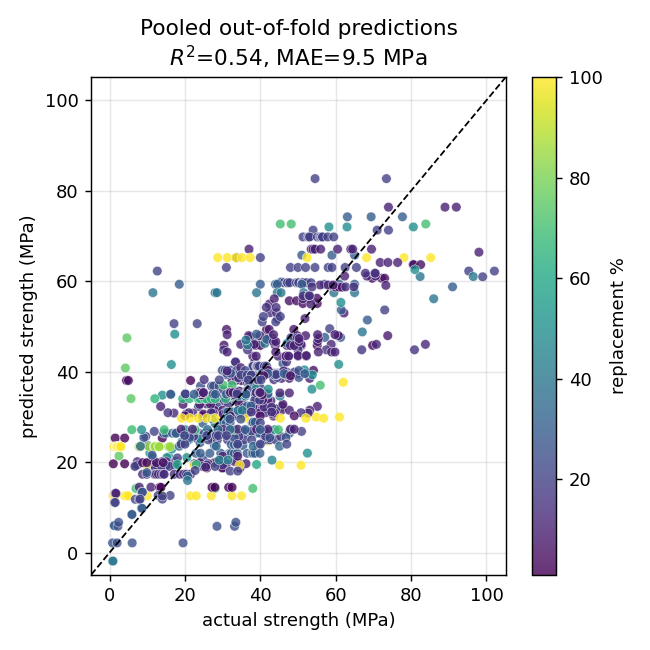
\includegraphics[width=\linewidth]{pred_vs_actual.png}
    \caption{Out-of-fold predictions.}
    \label{fig:pva}
  \end{subfigure}\hfill
  \begin{subfigure}{0.57\textwidth}
    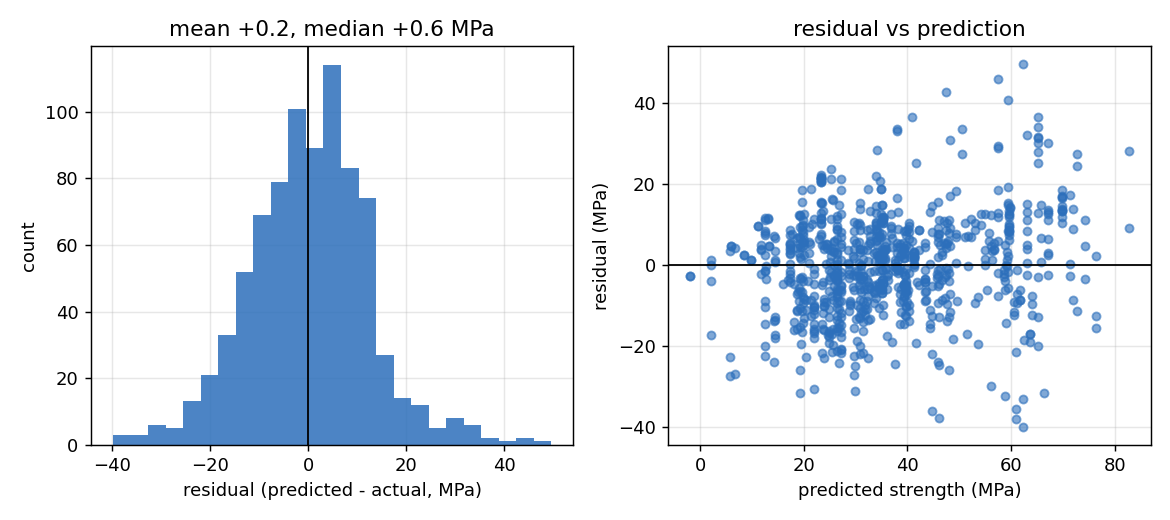
\includegraphics[width=\linewidth]{residuals.png}
    \caption{Residual diagnostics.}
    \label{fig:resid}
  \end{subfigure}
  \caption{Final model behaviour, from a single pooled 5-fold \texttt{GroupKFold}
  pass (\R{}~$=0.54$ pooled, versus the $0.448\pm0.175$ repeated-hold-out estimate
  quoted in the table above). Colour encodes replacement level. The dashed line is
  the ideal $y=x$; the points falling far below it at the right are the three
  high-strength papers.}
\end{figure}

\begin{figure}[H]
  \centering
  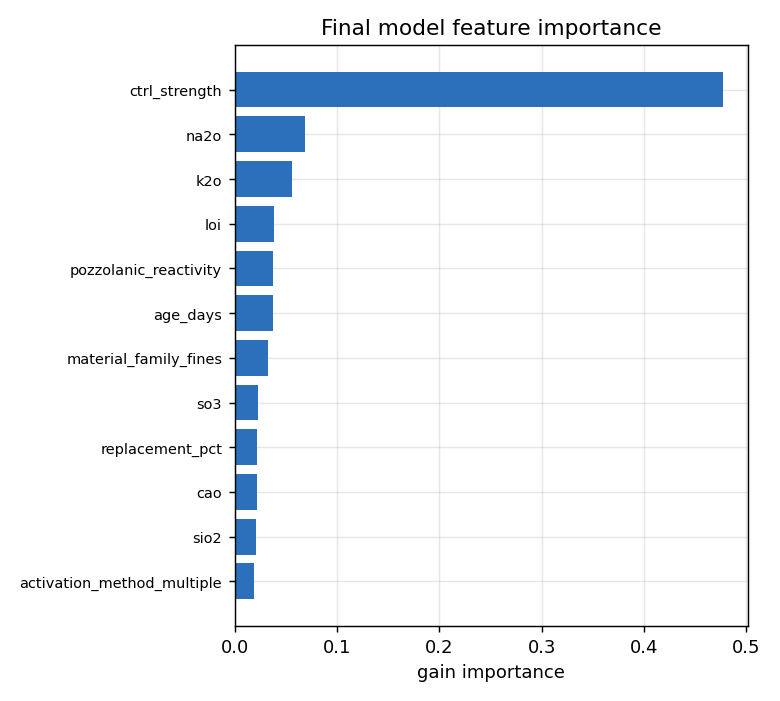
\includegraphics[width=0.65\textwidth]{feature_importance.png}
  \caption{Feature importance of the final model (top 12 of 37 columns after
  one-hot encoding). The paper's control strength dominates at 0.48; replacement
  level does not appear in the top eight.}
  \label{fig:imp}
\end{figure}

% ============================================================================
\section{Predicting the Optimal Replacement Level}
\label{sec:opt}
We derive the optimum as the replacement level maximizing the predicted 28-day
strength curve of the final model, swept over $0$--$50\%$ in $2.5$-point steps and
evaluated on held-out papers. It does not beat a naive prior: on the 32 held-out
papers with a reported optimum, the argmax approach gives MAE~$=14.0$ percentage
points against a mean-baseline of $8.6$.

Unlike the RHA study, the failure is \emph{not} degeneracy. That model collapsed to
a single constant for every paper; this one produces five distinct values spanning
$0$--$45\%$ (standard deviation $6.8$), and its predictions are concentrated where
the strength data says they should be---$9$ papers at $0\%$, $21$ at $5\%$, $11$ at
$7.5\%$. The model is behaving sensibly. The problem is the label.

\paragraph{The target is measuring two different things.}
Each paper supplies two candidate ``optima'': the one it \emph{reports in prose},
and the argmax of its \emph{own tabulated 28-day strengths}. On the 29 papers that
provide both, these disagree by \textbf{MAE~$=14.1$ percentage points} with a
correlation of only \textbf{$r=0.43$} (Figure~\ref{fig:opt}, right). The reported
optima average $18.8\%$; the empirical argmax of the same papers' own data averages
$5.4\%$, and for \textbf{18 of the 29 papers (62\%) the empirical optimum is $0\%$}
---their control mix is the strongest thing they measured.

The two labels therefore disagree with each other \emph{more} than our model
disagrees with either of them ($14.0$ against the reported optimum, $7.8$ against
the empirical one). This is not noise to be modelled away. A paper that recommends
``20\% RCP'' while its own table shows strength falling monotonically from 0\% is
not making an arithmetic error---it is optimizing something else: cost, CO$_2$
saving, workability, or an acceptable strength loss relative to a target grade. None
of those criteria are recorded in this dataset.

\paragraph{Neither label is beatable here, for different reasons.}
Against the reported optimum, the target encodes objectives the features do not
contain. Against the empirical optimum, the task is close to degenerate in the other
direction: since 62\% of papers peak at $0\%$, the constant predictor
``always~$0\%$'' already achieves MAE~$=5.05$ over the 39 papers with an empirical
optimum, better than our model's $7.81$ and exactly equal to the median prior. Predicting the strength-maximizing replacement level for
RCF is largely the trivial answer ``do not replace any cement,'' and the interesting
question---how much cement can be replaced for an acceptable strength penalty---is
not the question this label asks.

We therefore report the optimum task as a negative result with a diagnosis rather
than a number to improve: the corpus needs a defined optimality criterion before the
target is well-posed.

\begin{figure}[H]
  \centering
  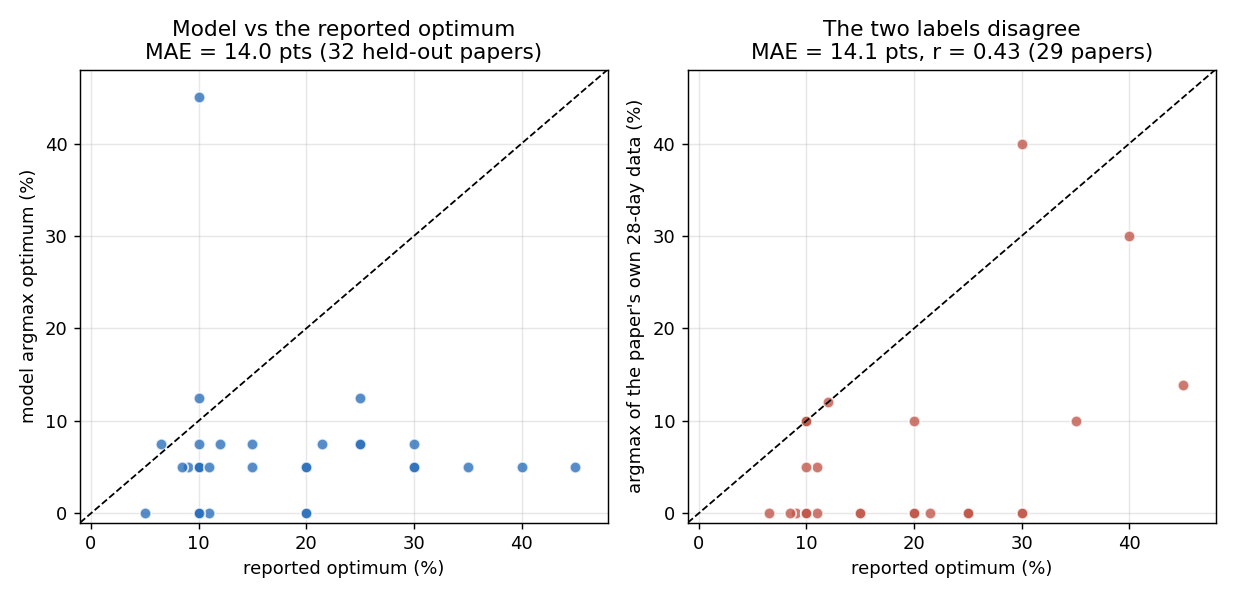
\includegraphics[width=0.92\textwidth]{optimum_scatter.png}
  \caption{\textbf{Left:} the model's argmax against each paper's reported optimum;
  MAE~$=14.0$ points over 32 held-out papers, worse than the $8.6$-point mean prior.
  \textbf{Right:} why. Each paper's reported optimum plotted against the argmax of
  its \emph{own} 28-day strength table---the two disagree by 14.1 points at
  $r=0.43$, with the reported values systematically higher. The label is not
  measuring strength maximization.}
  \label{fig:opt}
\end{figure}

% ============================================================================
\section{Comparison with the Rice-Husk-Ash Corpus}
\label{sec:cmp}
The two workbooks share a schema and were processed with deliberately parallel
pipelines, so the differences in Table~\ref{tab:cmp} are differences in the data and
the material, not in method.

\begin{table}[H]\centering\small
\caption{RHA versus RCF, from the two pipelines' own outputs.}
\label{tab:cmp}
\begin{tabular}{lrr}
\toprule
 & RHA & RCF \\
\midrule
Papers in the workbook & $79$ & $104$ \\
Recovered strength points & $756$ & $1825$ \\
Papers yielding points & $44$ & $85$ \\
Papers with a 0\% control (age-resolved) & $25$ & $49$ \\
Framing-C rows / papers & $335$ / $23$ & $823$ / $44$ \\
Papers peaking at an interior level & $42\%$ & $23\%$ \\
Does adding features help? & no (overfits) & yes \\
Final model \R{} (repeated grouped hold-out) & $0.50\pm0.20$ & $0.448\pm0.175$ \\
Final model MAE (MPa) & $10.1$ & $9.9$ \\
\bottomrule
\end{tabular}
\end{table}

The two final models land in the same place on MAE and are within noise of each
other on \R{}; the RCF model has the tighter spread, as one would expect from twice
the papers. But the two \R{} values are not measuring against the same ceiling---the
RCF task carries the $0.80$ noise ceiling of Section~\ref{sec:ceiling} because its
duplicate mixes are unresolvable, a limit the RHA corpus does not have---so the
apparent tie understates the RCF model.

Three further points are worth drawing out.

\textbf{RCF has roughly twice the usable data,} largely because the workbook ships a
pre-exploded Experimental Matrix alongside the packed grids. That extra sample size
is what flips the Study~3 result: feature groups that overfit at 23~papers earn
their place at 44.

\textbf{The materials behave differently.} An interior strength optimum is common in
RHA (42\% of papers) but the exception in RCF (23\%), where 71\% of papers are
strongest at the lowest replacement level tested. Rice husk ash is a genuinely
pozzolanic material that can improve strength at modest replacement; recycled
concrete powder mostly dilutes the binder. Any framing that presumes an interior
optimum is therefore a worse fit for RCF than for RHA. Both optimum-prediction
studies fail, but for different reasons, and the distinction matters: the RHA model
failed \emph{mechanically}, collapsing to a constant 7.5\% because its depth-2
monotone structure could not move an argmax; the RCF model behaves sensibly and
fails because the \emph{label} is ill-posed (Section~\ref{sec:opt}). Only the second
diagnosis points at the data collection rather than the model.

\textbf{Both corpora are limited by unrecorded mix descriptors, in different ways.}
In RHA the missing information is the base mix (cement grade, aggregate,
superplasticizer), which is why absolute strength is unpredictable across papers.
In RCF that problem persists \emph{and} is joined by a second one: the activation
treatment varies within a single (paper, level, age) coordinate and is recorded only
as free text, which is what produces the \R{}~$=0.80$ ceiling of
Section~\ref{sec:ceiling}. Structuring the per-mix activation and w/b columns is the
highest-value next step for this dataset---higher than any further modelling work.

% ============================================================================
\part*{Part II --- LLM Approach and the RCF Feature-Set Finding}
\label{sec:part2}

Part~II answers two further questions on the RCF corpus: does the same three-feature
recipe that won for RHA also win here, and can a general-purpose LLM predict RCF
strength the way Part~I's tree does?

\section{The Best Feature Set Is Not the Same as RHA's}
\label{sec:p2-features}
It is not. Section~\ref{sec:final}'s architecture search---model family $\times$ five
feature sets $\times$ duplicate handling $\times$ monotone constraints, 40
configurations, each on the same 40 repeated grouped hold-outs---found that
\texttt{base+cat+chem} (replacement, age, control strength, plus the four canonicalised
categoricals, pozzolanic reactivity, and the ten oxides) beats the bare three-feature
\texttt{base} set by $0.410$ vs $0.355$ \R{}, averaged over every other axis. The final
tuned model uses exactly that 18-feature set (Table in Section~\ref{sec:final}:
\R{}~$=0.448\pm0.175$, RMSE~$=12.9$, MAE~$=9.9$\,MPa).

This is the opposite of Part~I of the RHA report, where every added feature group made
generalisation \emph{worse} at 23 papers and the three base inputs won outright. The
difference is sample size, not the material: RCF's framing-C set has 44 papers against
RHA's 21--23, and Table~\ref{tab:cmp} already identifies this as what ``flips the
Study~3 result.'' The practical lesson is that there is no universal answer to which
features help---it must be re-established for each corpus, and here the answer is
chemistry and categoricals earn their place; for RHA they do not.

% ----------------------------------------------------------------------------
\section{LLM Approach: gpt-oss on the RCF Benchmark}
\label{sec:p2-llm}

\subsection{Setup}
Six papers were held out at the paper level, spanning the range of control strength in
the framing-C set (12.0 to 87.3\,MPa): papers 51, 81, 37, 19, 27 and 44, giving 56 test
points (the remaining 38 papers, 767 rows, are the training set). gpt-oss:120b-cloud is
given the same 18 inputs as the tuned XGBoost model above---\texttt{base+cat+chem}---so
the comparison in Section~\ref{sec:p2-direct} is on identical information, not just
identical rows. RCF has genuine repeat-specimen rows (the same paper, replacement level
and age measured more than once): 26 of the 56 test rows share a key with another row,
so predictions are matched to ground truth by a stable row index fixed once when the
benchmark was built, not by re-joining on those columns.

\paragraph{Reusing the RHA settings ablation.} The RHA report's Part~III ran a five-way
ablation of reproducibility settings (temperature~0 and a fixed seed; adding fully
greedy decoding; a JSON output schema; low reasoning effort; one prompt per paper) and
found that fully greedy decoding gave the smallest run-to-run spread and the best
accuracy, and that \emph{no} setting made the model deterministic. Rather than repeat
that five-way search on RCF's much larger training table, we apply its conclusion
directly: greedy decoding (temperature~0, fixed seed, \texttt{top\_k}\,=\,1,
\texttt{top\_p}\,=\,1, no repetition penalty, a fixed output cap), one fixed prompt, 15
runs, aggregated by per-point median in blocks of five. If RCF's data behaves
differently under this setting, that would already show up as a wider run-to-run spread
below.

\begin{center}
\begin{minipage}{0.92\linewidth}
\footnotesize
\begin{verbatim}
You are a concrete materials scientist predicting the compressive strength of
recycled-concrete-fines (RCF) blended concrete and mortar from published literature
data.

TRAINING DATA
Below are {n_train} measured data points from other papers, as CSV with a header row.
Each row is one (paper, RCF replacement %, curing age) combination. ctrl_strength is
that same paper's own 0% RCF (plain cement) strength AT THE SAME CURING AGE as the
row. Other columns describe the RCF powder: its chemistry (sio2, cao, al2o3, fe2o3,
mgo, so3, na2o, k2o, loi, amorphous_pct, as percentages), how it was processed and
activated (activation_method, processing_method), its mineralogy and material family,
and its pozzolanic reactivity. compressive_strength_mpa is the measured strength of
the blend. Learn how these inputs relate to compressive_strength_mpa.
--- BEGIN TRAINING CSV ---
{train_csv}
--- END TRAINING CSV ---

TASK
Predict compressive_strength_mpa for the {n_queries} query rows below. They come from
papers that are NOT in the training data. Each row states its paper_id; rows with the
same paper_id share one mix design. ctrl_strength is that paper's own 0% RCF strength
at that SAME curing age -- use it as that paper's baseline strength level at that age.

{queries}

OUTPUT FORMAT
Return only a JSON array of exactly {n_queries} numbers: one predicted compressive
strength in MPa per query, in query order (Query 1 first). No units, no text, no code
fence. Example for three queries: [12.3, 45.6, 30.1]
\end{verbatim}
\end{minipage}
\end{center}

\subsection{Results}
\label{sec:p2-llm-results}
Thirteen of the 15 runs returned a valid, complete answer; two returned the wrong
count of values and are excluded.

\begin{center}\small
\begin{tabular}{lrrr}
\toprule
& \R{} & RMSE (MPa) & MAE (MPa) \\
\midrule
Single run (13 valid; \R{} from $0.297$ to $0.875$) & $0.659\pm0.195$ & $12.14\pm3.51$ & $8.39\pm2.58$ \\
\rowcolor{green!12}Median of 5 runs, block 1 & $\mathbf{0.753}$ & $10.72$ & $6.60$ \\
\rowcolor{green!12}Median of 5 runs, block 2 & $\mathbf{0.847}$ & $8.43$ & $5.80$ \\
\bottomrule
\end{tabular}
\end{center}

\noindent The pattern already established for RHA holds here too: a single run can land
almost anywhere (\R{} $0.30$ to $0.88$), and the per-point median of five runs is both
more accurate and more stable. The two independent five-run medians agree to a typical
2.35\,MPa per point (worst point 8.30\,MPa)---wider than RHA's 1\,MPa agreement, which is
expected given RCF's larger, noisier training table (767 rows and free-text categorical
fields, against RHA's few hundred rows).

\subsection{Direct Comparison with the Tuned XGBoost Model}
\label{sec:p2-direct}
The Section~\ref{sec:final} XGBoost model (same hyper-parameters, monotone in age and
control strength) was trained on the identical 767 training rows and scored on the
identical 56 test rows.

\begin{center}\small
\begin{adjustbox}{max width=\linewidth}
\begin{tabular}{lrrrl}
\toprule
Model & \R{} & RMSE (MPa) & MAE (MPa) & Same answer every time? \\
\midrule
XGBoost (final model) & $0.737$ & $11.07$ & $6.82$ & yes (identical) \\
\rowcolor{green!12}gpt-oss, median of 5 (better block) & $\mathbf{0.847}$ & $\mathbf{8.43}$ & $\mathbf{5.80}$ & within $\approx2$\,MPa \\
gpt-oss, median of 5 (other block) & $0.753$ & $10.72$ & $6.60$ & \\
gpt-oss, single run & $0.659\pm0.195$ & $12.14\pm3.51$ & $8.39\pm2.58$ & no \\
\bottomrule
\end{tabular}
\end{adjustbox}
\end{center}

\noindent \textbf{This reverses the RHA finding.} On RHA's benchmark, the three-input
XGBoost model beat gpt-oss's median-of-5 (\R{}~$0.778$ vs $0.703$). On RCF's benchmark,
gpt-oss's median-of-5 beats XGBoost in both blocks (\R{}~$0.75$--$0.85$ vs $0.737$), and
even a single gpt-oss run is competitive. By strength band (papers sorted by control
strength; MAE in MPa, gpt-oss column uses the better block):

\begin{center}\small
\begin{tabular}{lrrrr}
\toprule
Paper (control strength) & $N$ & XGBoost MAE & gpt-oss MAE & gpt-oss bias \\
\midrule
51 (12.0\,MPa) & 6 & $2.09$ & $2.26$ & $+2.26$ \\
81 (18.7\,MPa) & 9 & $2.69$ & $\mathbf{1.88}$ & $+0.72$ \\
37 (29.1\,MPa) & 12 & $2.96$ & $2.40$ & $-0.93$ \\
19 (40.0\,MPa) & 14 & $2.88$ & $3.79$ & $+3.79$ \\
27 (56.4\,MPa) & 6 & $17.56$ & $26.98$ & $+26.98$ \\
44 (87.3\,MPa) & 9 & $\mathbf{18.21}$ & $\mathbf{10.61}$ & $+7.28$ \\
\bottomrule
\end{tabular}
\end{center}

\noindent Both models are accurate (MAE 2--4\,MPa) on four of the six papers and both
struggle on the same two. Paper~44, the highest-control paper, is where gpt-oss's
advantage is concentrated: XGBoost under-predicts it by 18.2\,MPa on average (bias
$-18.21$; this is the same high-control failure mode documented for RHA, where grouped
validation always places an extreme paper wholly in the test fold), while gpt-oss's
error there is little more than half as large (MAE $10.61$) and in the opposite
direction (over-, not under-predicting). Paper~27 is hard for \emph{both} models---and
harder for gpt-oss---despite its control strength being unremarkable (56.4\,MPa); its
own strength range is 17--73.5\,MPa, an unusually wide spread for one paper, consistent
with the unresolved duplicate-mix and activation-labelling issue that already caps this
whole corpus at the \R{}~$=0.80$ noise ceiling of Section~\ref{sec:ceiling}.

\paragraph{Why might gpt-oss do better here than on RHA?} We did not run a controlled
test of this, so it is offered as a hypothesis, not a finding: RCF's winning feature set
includes free-text categoricals (activation method, processing method, mineralogy) and
ten oxide percentages, which is exactly the feature growth that helps here but hurt on
RHA (Section~\ref{sec:p2-features}). An LLM can bring semantic prior knowledge to values
like ``ball milling'' or ``high pozzolanic reactivity'' that a one-hot-encoded tree
cannot; RHA's winning feature set was only three numbers, where a tree has no
disadvantage. This is consistent with, but does not prove, the pattern in this section.

% ----------------------------------------------------------------------------
\section{Part II Summary}
\label{sec:p2-summary}
\begin{itemize}\itemsep3pt
  \item \textbf{The best feature set is corpus-specific.} RHA's three base inputs
        overfit at 23 papers; RCF's chemistry and categorical features earn their place
        at 44 papers, lifting \R{} from $0.355$ to $0.410$ on average, and $0.448\pm0.175$
        for the final tuned model.
  \item \textbf{gpt-oss is not reproducible here either}, for the same reason found on
        RHA: a single run's \R{} ranges from $0.30$ to $0.88$; the per-point median of
        five runs is both more accurate and stable (agreement $\approx2$\,MPa per point).
  \item \textbf{On the same 56 test points, gpt-oss's median-of-5 beats the tuned
        XGBoost model} (\R{}~$0.75$--$0.85$ vs $0.737$)---the opposite ranking from RHA,
        where XGBoost won. The gap is concentrated in the paper with the highest control
        strength, which XGBoost badly under-predicts and gpt-oss handles much better.
\end{itemize}

% ============================================================================
\part*{Part III --- RCF up to 60\,MPa: What Actually Works}
\label{sec:rcf-p3}

Part~III redoes the RCF analysis on the range we care about---samples up to
60\,MPa---and asks, without assuming the rice-husk-ash (RHA) answer transfers, which
method and which inputs actually work. It ends with a like-for-like comparison of the
best ML model and an LLM on the same held-out papers, given exactly the same
information.

% ----------------------------------------------------------------------------
\section{The Data After Removing Samples Above 60\,MPa}
\label{sec:rcf-p3-data}
Every row whose measured strength exceeds 60\,MPa is dropped, control rows included.

\begin{center}\small
\begin{adjustbox}{max width=\linewidth}
\begin{tabular}{lrr}
\toprule
 & All samples & $\leq60$\,MPa \\
\midrule
Parsed data points / papers & 1825 / 85 & 1675 / 83 \\
Rows with a resolved curing age & 1284 & 1165 \\
Modelling set: blends with a same-age control / papers & 823 / 44 & \textbf{688 / 41} \\
Spread of the modelling target (SD) & 18.1\,MPa & 14.1\,MPa \\
\bottomrule
\end{tabular}
\end{adjustbox}
\end{center}

\noindent The filter removes 150 rows from 27 papers and costs 3 papers in the modelling
set. Every model below is trained on those 688 rows and scored the same way as in
Part~I: \textbf{repeated grouped hold-out, 30\% of papers held out, 40 repeats}, so no
paper is ever in both training and test. Because the filter also narrows the spread of
the target (18.1 $\to$ 14.1\,MPa), \R{} values here are not comparable with Part~I's;
RMSE and MAE, in MPa, are.

% ----------------------------------------------------------------------------
\section{Which ML Method Works Best}
\label{sec:rcf-p3-model}
Nine candidates, all on the same rows, features and splits.

\begin{center}\small
\begin{adjustbox}{max width=\linewidth}
\begin{tabular}{lrrr}
\toprule
Model & \R{} & RMSE (MPa) & MAE (MPa) \\
\midrule
\rowcolor{green!12}HistGradientBoosting & $\mathbf{0.269\pm0.227}$ & $\mathbf{11.30}$ & $\mathbf{8.60}$ \\
ExtraTrees & $0.257\pm0.216$ & $11.40$ & $8.85$ \\
Random Forest & $0.256\pm0.246$ & $11.37$ & $8.66$ \\
XGBoost & $0.244\pm0.238$ & $11.48$ & $8.74$ \\
GradientBoosting & $0.224\pm0.278$ & $11.59$ & $8.75$ \\
Mean baseline & $-0.112\pm0.163$ & $14.08$ & $11.56$ \\
Stack (RF + XGB + Ridge) & $-8.9\pm56.5$ & $17.80$ & $11.50$ \\
Ridge & $-845\pm5146$ & $93.3$ & $43.3$ \\
MLP (64, 32) & $-2.0\times10^{5}$ & $1036$ & $393$ \\
\bottomrule
\end{tabular}
\end{adjustbox}
\end{center}

\noindent The four tree ensembles are within noise of each other, and
\textbf{HistGradientBoosting is the best of them---XGBoost, the RHA winner, is fourth}.
Linear Ridge and the MLP fail completely: with 18 sparse inputs and papers whose strength
levels differ by an order of magnitude, an unconstrained linear or neural fit extrapolates
wildly on held-out papers. The stack inherits Ridge's failures. Only the tree ensembles
beat predicting the average.

% ----------------------------------------------------------------------------
\section{Which Features Earn Their Place}
\label{sec:rcf-p3-features}
Feature groups added to the base inputs (replacement level, curing age, control
strength), all with XGBoost so the rows are comparable with Part~I.

\begin{center}\small
\begin{adjustbox}{max width=\linewidth}
\begin{tabular}{lrrr}
\toprule
Feature set & \R{} & RMSE (MPa) & MAE (MPa) \\
\midrule
\rowcolor{green!12}all structured & $\mathbf{0.244\pm0.238}$ & $\mathbf{11.48}$ & $8.74$ \\
base + all numeric & $0.241\pm0.254$ & $11.49$ & $8.75$ \\
base + categorical & $0.224\pm0.241$ & $11.63$ & $8.85$ \\
all + MiniLM text embeddings & $0.216\pm0.229$ & $11.70$ & $8.91$ \\
base + chemistry & $0.205\pm0.277$ & $11.73$ & $8.85$ \\
all + TF-IDF text & $0.203\pm0.241$ & $11.80$ & $9.02$ \\
base + fineness & $0.181\pm0.254$ & $11.94$ & $9.11$ \\
base + processing & $0.181\pm0.287$ & $11.93$ & $9.06$ \\
base [replacement, age, control] & $0.142\pm0.299$ & $12.21$ & $9.05$ \\
base + mix descriptors & $0.109\pm0.313$ & $12.42$ & $9.21$ \\
\bottomrule
\end{tabular}
\end{adjustbox}
\end{center}

\begin{figure}[tbp]
  \centering
  \begin{subfigure}{0.49\textwidth}
    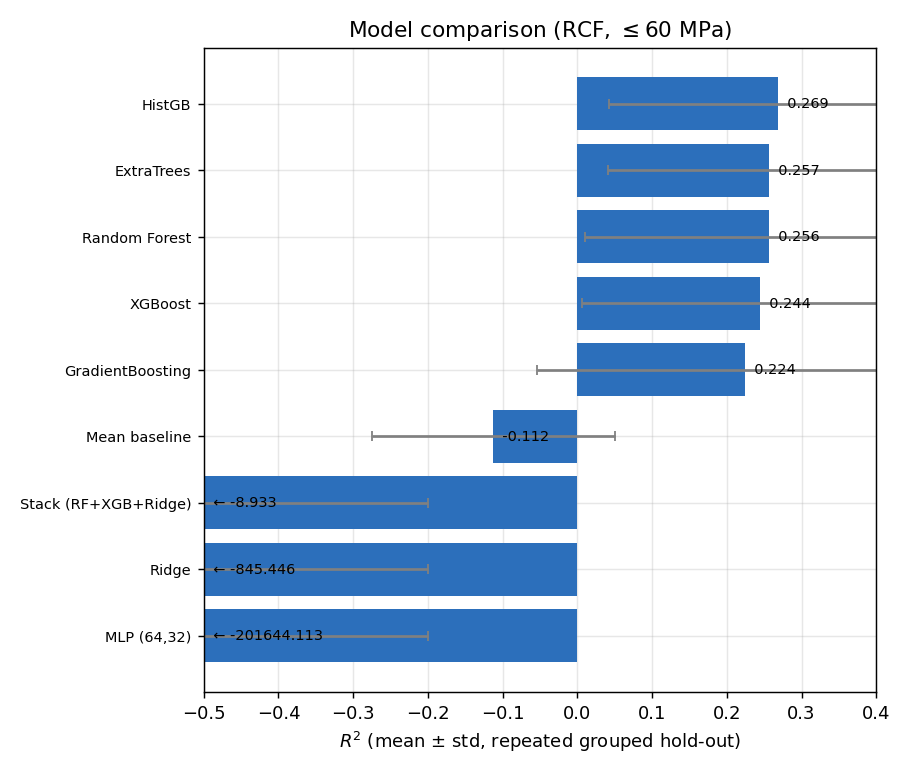
\includegraphics[width=\linewidth]{pipeline_rcf/out_le60/figs/abl_model.png}
    \caption{Model comparison.}
  \end{subfigure}\hfill
  \begin{subfigure}{0.49\textwidth}
    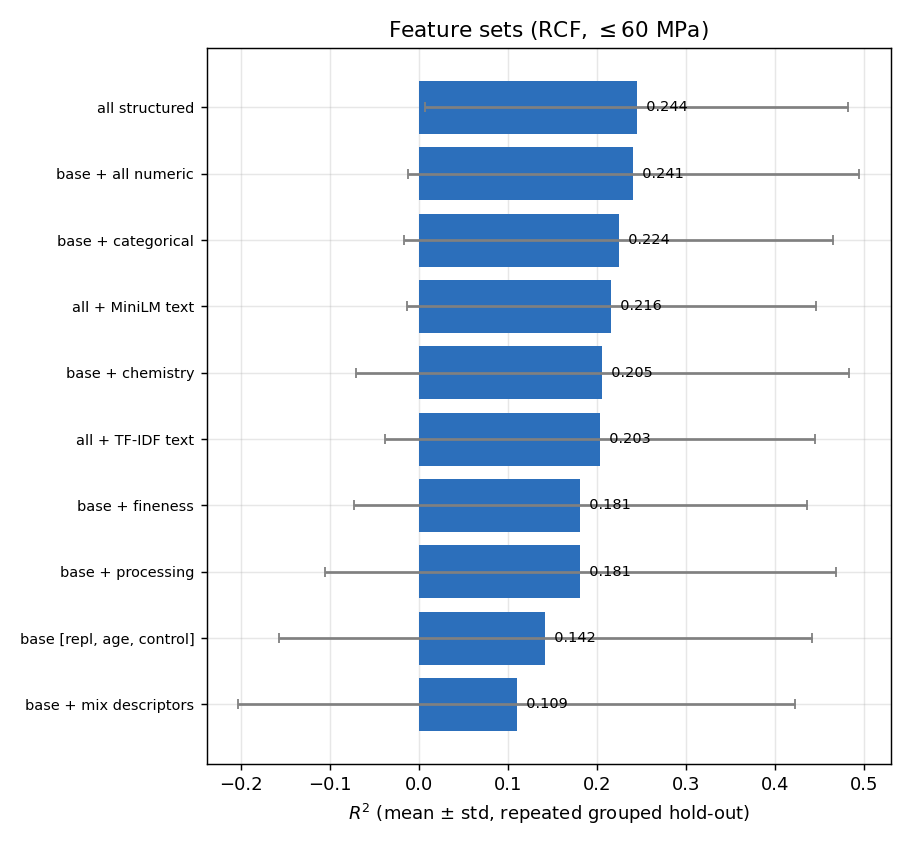
\includegraphics[width=\linewidth]{pipeline_rcf/out_le60/figs/abl_features.png}
    \caption{Feature sets.}
  \end{subfigure}
  \caption{RCF at $\leq60$\,MPa: which model and which features help.}
  \label{fig:rcf-p3-abl}
\end{figure}

\noindent \textbf{This is the clearest difference from RHA.} On RHA, the three base
inputs were as good as anything and added feature groups only added noise. On RCF,
describing the powder genuinely helps: the base set alone scores 0.142, and adding the
material descriptors lifts it to 0.244---a gain larger than the gap between any two tree
models. Text embeddings of the papers' free-text fields do not beat the structured
columns. The plain reason is sample size: RCF's modelling set has 41 papers against
RHA's 21, so there are enough papers to support more inputs.

The architecture search (model $\times$ feature set $\times$ duplicate handling $\times$
monotone, 40 configurations) confirms this and picks a slightly leaner set: HistGB with
\emph{base + categorical + fineness} at \R{}~$=0.285$, ahead of the same model on all
structured features (0.269) and on the base set (0.266). Chemistry, which the full-data
Part~I favoured, is \emph{not} in the $\leq60$\,MPa winner.

% ----------------------------------------------------------------------------
\section{Does the Control Strength Help?}
\label{sec:rcf-p3-control}
Yes---it is the single most valuable input, exactly as on RHA.

\begin{center}\small
\begin{adjustbox}{max width=\linewidth}
\begin{tabular}{lrrr}
\toprule
Target framing & \R{} & RMSE (MPa) & Rows / papers \\
\midrule
\rowcolor{green!12}C: blend strength given the paper's control & $\mathbf{0.244\pm0.238}$ & $11.48$ & 688 / 41 \\
A: absolute strength, no control & $-0.130\pm0.216$ & $15.59$ & 1165 / 56 \\
B: strength relative to the control & $-0.162\pm0.204$ & --- & 688 / 41 \\
\bottomrule
\end{tabular}
\end{adjustbox}
\end{center}

\noindent Without the control strength the model is worse than predicting the corpus
average; with it, the problem becomes learnable. Predicting the \emph{ratio} to the
control (framing B) does not work either. In the final model, control strength carries by
far the largest importance (0.887, against 0.296 for replacement level).

% ----------------------------------------------------------------------------
\section{Missing Values and Physics Constraints}
\label{sec:rcf-p3-priors}
\begin{center}\small
\begin{adjustbox}{max width=\linewidth}
\begin{tabular}{lrr@{\hskip 2em}lrr}
\toprule
Missing values & \R{} & RMSE & Physics prior & \R{} & RMSE \\
\midrule
\rowcolor{green!12}median imputation & $\mathbf{0.249}$ & $11.42$ & \cellcolor{green!12}monotone in age, control & \cellcolor{green!12}$\mathbf{0.213}$ & \cellcolor{green!12}$11.71$ \\
native (no imputation) & $0.244$ & $11.48$ & plain & $0.142$ & $12.21$ \\
KNN imputation & $0.214$ & $11.70$ & log target + monotone & $0.118$ & $12.29$ \\
MICE imputation & $0.192$ & $11.89$ & log target & $0.116$ & $12.36$ \\
\bottomrule
\end{tabular}
\end{adjustbox}
\end{center}

\noindent Missing-value handling barely matters: letting the tree handle gaps natively and
filling them with column medians are equivalent, while the cleverer imputers (KNN, MICE)
are slightly worse. \textbf{Requiring strength to rise with curing age and with the
paper's control strength is worth more than any other single choice}: \R{} goes from
0.142 to 0.213 on the base inputs, and the constraint survives into the tuned model.
Log-transforming the target hurts.

% ----------------------------------------------------------------------------
\section{The Final ML Model}
\label{sec:rcf-p3-final}
Combining the winners and tuning the hyper-parameters:

\begin{center}\small
\begin{adjustbox}{max width=\linewidth}
\begin{tabular}{ll}
\toprule
Model & HistGradientBoosting, depth 2, learning rate 0.03, 300 iterations \\
Features (18) & replacement \%, curing age, control strength; activation method, \\
 & processing method, mineralogy, material family, pozzolanic reactivity; \\
 & d10, d50, d90, mean particle size, specific surface, BET surface, Blaine, \\
 & specific gravity, bulk density, water absorption \\
Constraint & strength non-decreasing in curing age and in control strength \\
\midrule
Performance & \R{}~$=\mathbf{0.308\pm0.187}$, RMSE~$=\mathbf{11.02}$\,MPa, MAE~$=\mathbf{8.47}$\,MPa \\
Mean baseline & \R{}~$=-0.112$, RMSE~$=14.08$\,MPa, MAE~$=11.56$\,MPa \\
Pooled 5-fold grouped & \R{}~$=0.319$, MAE~$=8.82$\,MPa (optimistic; single split) \\
\bottomrule
\end{tabular}
\end{adjustbox}
\end{center}

\noindent The model explains about a third of the variation between held-out papers, with
a typical error of 8.5\,MPa on a target whose spread is 14.1\,MPa. That is honest but
modest, and Part~I's diagnosis still applies: many (paper, level, age) cells hold several
distinct mixes whose treatment the dataset does not record, so a sizeable part of the
remaining error is irreducible from these columns.

\begin{figure}[tbp]
  \centering
  \begin{subfigure}{0.48\textwidth}
    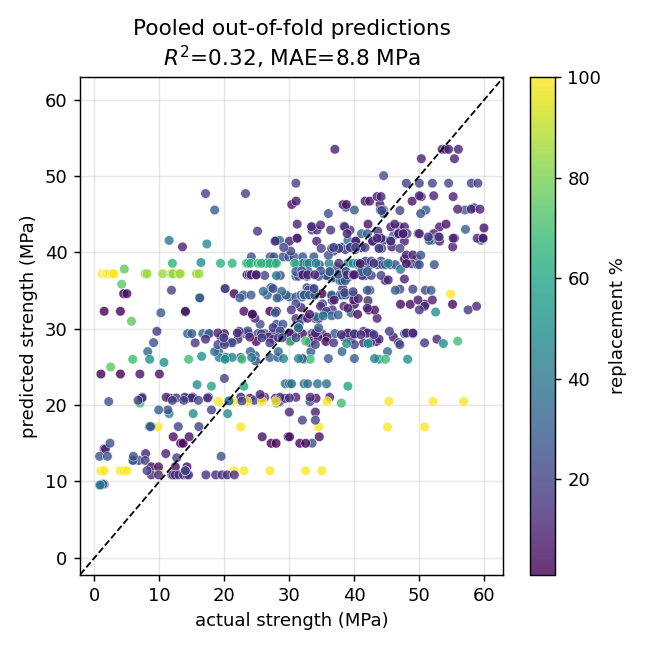
\includegraphics[width=\linewidth]{pipeline_rcf/out_le60/figs/pred_vs_actual.png}
    \caption{Out-of-fold predictions.}
  \end{subfigure}\hfill
  \begin{subfigure}{0.48\textwidth}
    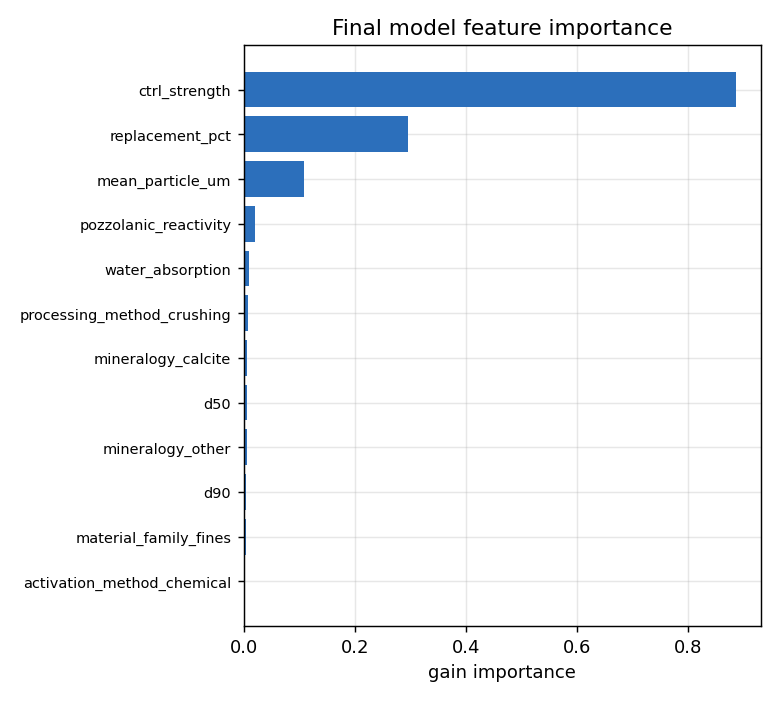
\includegraphics[width=\linewidth]{pipeline_rcf/out_le60/figs/feature_importance.png}
    \caption{Feature importance.}
  \end{subfigure}
  \caption{Final RCF model on the $\leq60$\,MPa data.}
  \label{fig:rcf-p3-final}
\end{figure}

% ----------------------------------------------------------------------------
\section{The LLM Approach}
\label{sec:rcf-p3-llm}
Six papers spanning the control-strength range (12 to 60\,MPa) are held out: papers 51,
81, 37, 19, 80 and 91, giving \textbf{59 test points}; the other 35 papers (629 rows) are
training data. Four of the six are the papers used in Part~II; papers 27 and 44 had to be
replaced because the $\leq60$\,MPa filter leaves paper 27 with 2 rows and removes paper 44
entirely.

gpt-oss:120b-cloud receives the 629 training rows as CSV in one fixed prompt and returns a
JSON array of 59 numbers. Settings are the greedy ones established in the RHA study
(temperature 0, fixed seed, top-$k$ 1, top-$p$ 1). The prompt was run \textbf{15 times};
answers were checked and retried, and all 15 were valid (14 on the first attempt). Each
call takes about 32\,s.

\begin{center}\small
\begin{adjustbox}{max width=\linewidth}
\begin{tabular}{lrrr}
\toprule
gpt-oss on the 59 held-out points & \R{} & RMSE (MPa) & MAE (MPa) \\
\midrule
Single run (mean of 15, $\pm$ SD) & $0.204\pm0.426$ & $13.13$ & $9.26$ \\
\quad worst / best single run & $-0.624$ / $0.852$ & & \\
Median of 5 runs (three blocks) & $0.560$ / $0.666$ / $0.464$ & $10.14$ / $8.83$ / $11.19$ & $6.76$ / $5.46$ / $7.53$ \\
\rowcolor{green!12}Median of all 15 runs & $\mathbf{0.602}$ & $\mathbf{9.34}$ & $\mathbf{6.29}$ \\
\bottomrule
\end{tabular}
\end{adjustbox}
\end{center}

\noindent A single gpt-oss run is unreliable on RCF: \R{} ranges from $-0.62$ to $0.85$
across runs of the identical prompt, and a typical individual prediction moves by 9\,MPa
between runs. Taking the per-point median of several runs is essential, and with all 15
runs pooled the model reaches \R{}~$=0.602$. This matches the RHA finding that the median
of repeated runs, not a single call, is what should be deployed.

% ----------------------------------------------------------------------------
\section{ML versus LLM on the Same Test Points}
\label{sec:rcf-p3-vs}
Both methods were given \emph{exactly} the same information, and this was enforced rather
than assumed. The parity rules, recorded in
\path{pipeline_rcf/out_llm_le60/parity_manifest.json}, are:

\begin{itemize}\itemsep1pt
  \item the same 6 held-out papers and the same 59 test rows, in one fixed order;
  \item the same 629 training rows;
  \item the same 18 input columns --- the prompt's training CSV and query lines contain
        exactly the columns the ML model is fitted on, and nothing else;
  \item \textbf{no identifiers for either method}: paper id, row id, mix id and data
        source are withheld from the prompt because the ML model never sees them.
        Predictions are matched by query order alone;
  \item the measured strength of a test row is shown to neither method.
\end{itemize}

\begin{center}\small
\begin{adjustbox}{max width=\linewidth}
\begin{tabular}{lrrrl}
\toprule
Method (identical inputs, identical 59 test points) & \R{} & RMSE & MAE & Repeatable? \\
\midrule
\rowcolor{green!12}HistGradientBoosting (the final model) & $\mathbf{0.789}$ & $\mathbf{7.03}$ & $\mathbf{5.52}$ & yes, identical \\
gpt-oss, median of 15 runs & $0.602$ & $9.34$ & $6.29$ & $\approx2.5$\,MPa per point \\
gpt-oss, single run & $0.204\pm0.426$ & $13.13$ & $9.26$ & no \\
\bottomrule
\end{tabular}
\end{adjustbox}
\end{center}

\noindent \textbf{The ML model wins on equal terms}, and it is also deterministic and
runs in milliseconds rather than 32\,s per call. Per paper, the two are close on four of
the six and differ on two: gpt-oss is better on papers 91 (MAE 2.9 vs 9.8) and 37 (2.6 vs
3.6), while HistGB is better on 19 (2.4 vs 4.5) and 80 (8.7 vs 15.4).

\paragraph{What the paper identifier was worth.} A diagnostic run---\emph{not} part of the
comparison above---put \texttt{paper\_id} back into the prompt, which is what the earlier
RCF benchmark of Part~II and the RHA study both did while their ML models never received
it. With that single extra column the LLM improves sharply:

\begin{center}\small
\begin{adjustbox}{max width=\linewidth}
\begin{tabular}{lrrr}
\toprule
gpt-oss, 59 test points & Single run \R{} & Median-of-runs \R{} & Per-point spread \\
\midrule
paper id hidden (parity, 15 runs) & $0.204\pm0.426$ & $0.602$ & $9.1$\,MPa \\
paper id visible (diagnostic, 5 runs) & $0.668\pm0.089$ & $0.743$ & $3.6$\,MPa \\
\bottomrule
\end{tabular}
\end{adjustbox}
\end{center}

\noindent The identifier carries no strength information, but it tells the model which
query rows belong to the same paper, so it can anchor each block on that paper's control
strength. Without it the model sometimes mixes the blocks up---predicting about 14\,MPa
for a paper whose control is 47.7\,MPa. A tree model cannot exploit such grouping at all,
so giving it to the LLM alone makes the comparison unfair; that is why the headline table
withholds it. It also means the LLM-favourable margins reported in Part~II should be read
with this caveat.

% ----------------------------------------------------------------------------
\section{Can We Predict the Optimal Replacement Level?}
\label{sec:rcf-p3-opt}
No. Of the 41 papers in the modelling set, 30 report an optimum. Sweeping the final model
over replacement levels and taking the best predicted strength gives
\textbf{MAE~$=12.7$ percentage points, against 8.9 for simply predicting the corpus mean
optimum}. The predicted optima take only 4 distinct values spanning 0--10\%, while the
reported ones range from 5 to 45\% (mean 18\%, SD 10.6).

Two deeper problems make the target ill-posed on this corpus, both unchanged from Part~I:
the 27 papers that report both an optimum and a measurable best mix disagree by
\textbf{14.4 percentage points on average} ($r=0.46$), and for \textbf{66\% of papers the
strongest mix actually measured is the 0\% control}---that is, RCF never helped, so an
"optimum" is a matter of definition rather than a measured fact. We recommend not
reporting an optimum-prediction model for RCF.

% ----------------------------------------------------------------------------
\section{What We Should Use for RCF}
\label{sec:rcf-p3-reco}
\begin{enumerate}\itemsep2pt
  \item \textbf{Model:} HistGradientBoosting, depth 2, with strength required to rise with
        curing age and control strength. XGBoost is a close second; Ridge and neural nets
        are not usable here.
  \item \textbf{Inputs:} the paper's own control strength at the same age is essential,
        together with replacement level and age; add the categorical descriptors and the
        fineness measurements. Unlike RHA, these extra columns genuinely help.
  \item \textbf{Missing values:} leave them to the model or fill with column medians;
        do not bother with KNN or MICE.
  \item \textbf{Validation:} always group by paper. Expect \R{}~$\approx0.31$ and a
        typical error of 8.5\,MPa on unseen papers.
  \item \textbf{The LLM is not the primary tool for RCF.} On identical inputs it is
        clearly behind the tuned model, needs the median of several runs to be stable at
        all, and costs about 32\,s per call. It is a reasonable fallback where no trained
        model exists, and it was competitive only when given a paper identifier the ML
        model did not have.
  \item \textbf{Do not report an optimal replacement level} from this data.
\end{enumerate}

\noindent \textbf{Does the RHA recipe transfer?} Partly. The one thing that transfers
completely is the control strength: on both corpora it is what makes the problem
learnable, and physics constraints help on both. What does \emph{not} transfer is the
rest: RCF prefers HistGradientBoosting over XGBoost, and RCF rewards the extra material
descriptors that RHA punished, because RCF has roughly twice as many papers. Running
RHA's exact recipe on RCF---XGBoost on the three base inputs with monotone
constraints---scores \R{}~$=0.213$ against 0.285 for RCF's own best architecture, so
transferring the recipe unchanged would give away about a quarter of the achievable
score.

\end{document}
